\chapter{Results and Discussion}\label{ch:resultsanddiscussion}

\section{Hydrogen Lowest-Energy States}\label{sec:hydrogengroundstates}

\subsection{Atomic and Molecular Hartree-Fock Methods}\label{subsec:hartreeanalyticresults}


Figure \ref{fig:hydrogenatomicgroundstates} below shows orbital electron wavefunctions calculated for the six valid $s$, $p$, and $d$-type ($l=0$, $l=1$, and $l=2$ respectively) lowest-energy Hydrogen states, found using the atomic Hartree-Fock approximation. Here, the shapes of each orbital closely match existing exact solutions for Hydrogen, found by decomposing the Schrödinger-equation wavefunction into radial and spherical-harmonic components \cite{nalewajski_perspectives_2012}\cite{walczak_hydrogen_2013}. The orbitals displayed are the real-valued components of each wavefunction, each of which occupies very distinct locations around the atomic centre, and has clear boundaries between positive and negative amplitude points.


\begin{figure}[h!]
\begin{center}
\hspace*{-2.7cm}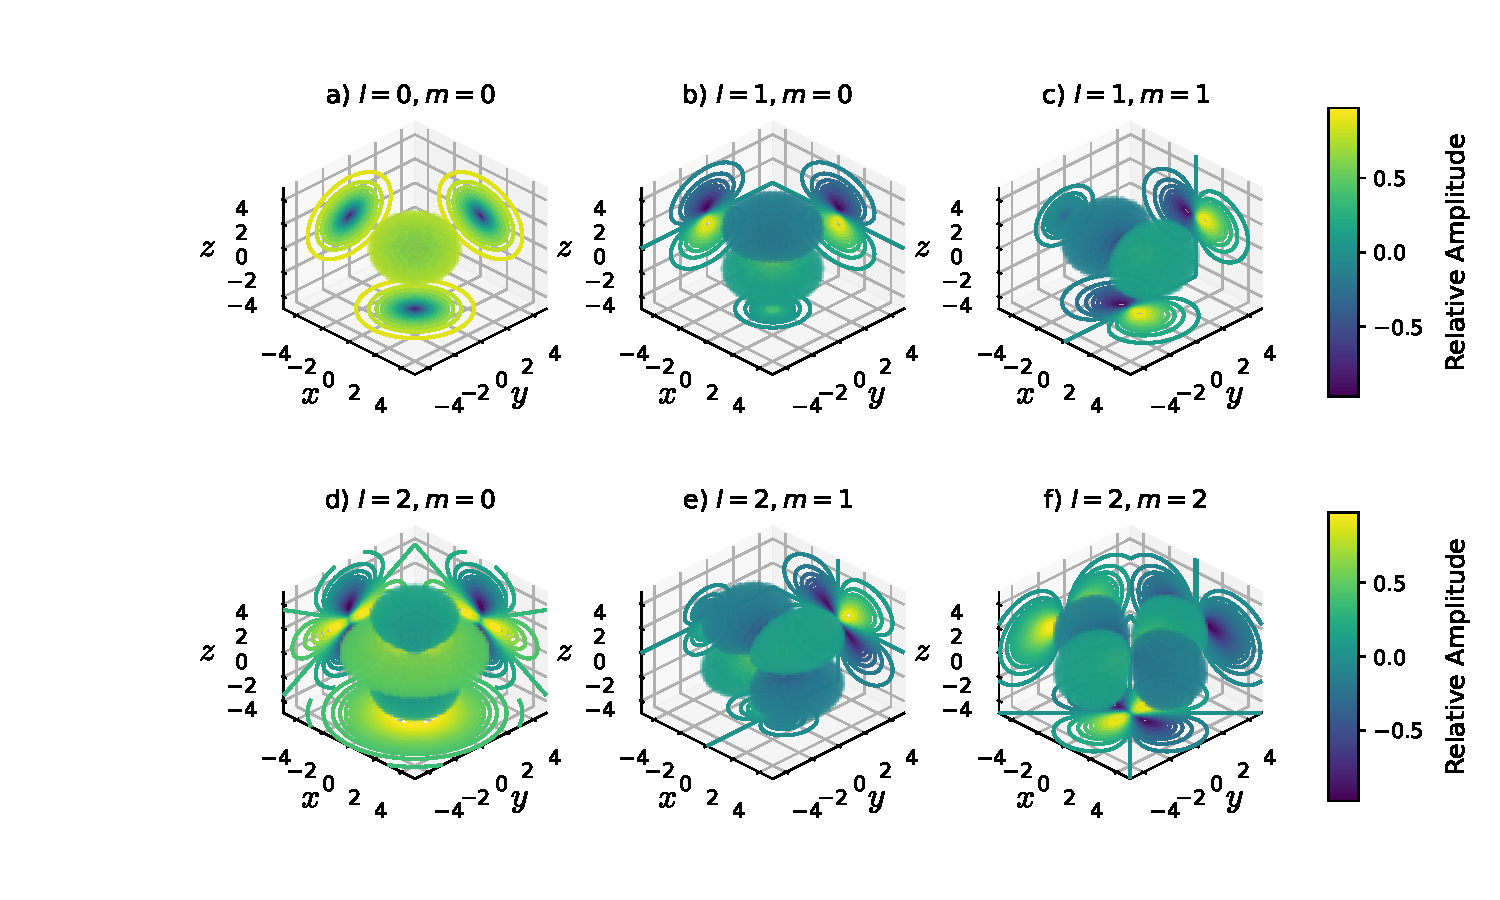
\includegraphics[width=1.2\linewidth, trim={0 0 0 1cm}, clip]{figures/HydrogenAtomicSTypeStates.pdf}\vspace*{-1cm}
\end{center}
\caption{Orbital electron wavefunctions for the lowest-energy Hydrogen states with azimuthal quantum numbers from $l=0$ to $l=2$, calculated using the atomic Hartree-Fock approximation. These closely match known Hydrogen orbitals calculated analytically \cite{walczak_hydrogen_2013}. Displayed using a 3D scatterplot, and filtered to display real-valued wavefunction components greater than 10\% relative amplitude. Calculated using a domain of (50x50x50) position cells.}
\label{fig:hydrogenatomicgroundstates}
\end{figure}
\clearpage

Figure \ref{fig:hydrogenhartreeatomicmolecular} below shows the first three electron orbital wavefunctions for s-type ($l=0$, $m=0$) Hydrogen, calculated with both the atomic and molecular forms of the Hartree-Fock approximation. Both methods produced identical wavefunctions with expected shapes, and so only the atomic result has been plotted. This confirms that the hydrogenic components of the molecular Hartree-Fock method ($\boldsymbol{S}$, $\boldsymbol{T}$, and $\boldsymbol{V}$) have been implemented correctly in the project script, and allows us to continue to more complex methods.\\

The first six ground-state eigenvalues found with these methods were also identical to one-another, and were $E_1=-13.606$ $eV$, $E_2=-3.401$ $eV$, $E_3=-1.512$ $eV$, $E_4=-0.850$ $eV$, $E_5=-0.544$ $eV$, and $E_6=-0.313$ $eV$. Of these, the first five closely match their exact Bohr model values of $-13.6/n^2$ $eV$, however the sixth and further energies diverge quickly \cite{pinke_origin_2025}. Therefore, the Hartree-Fock methods both give a reasonable approximation of the first few low-energy states, but become inaccurate quickly for those with higher energies. 

\begin{figure}[h!]
\begin{center}
\hspace*{-2.7cm}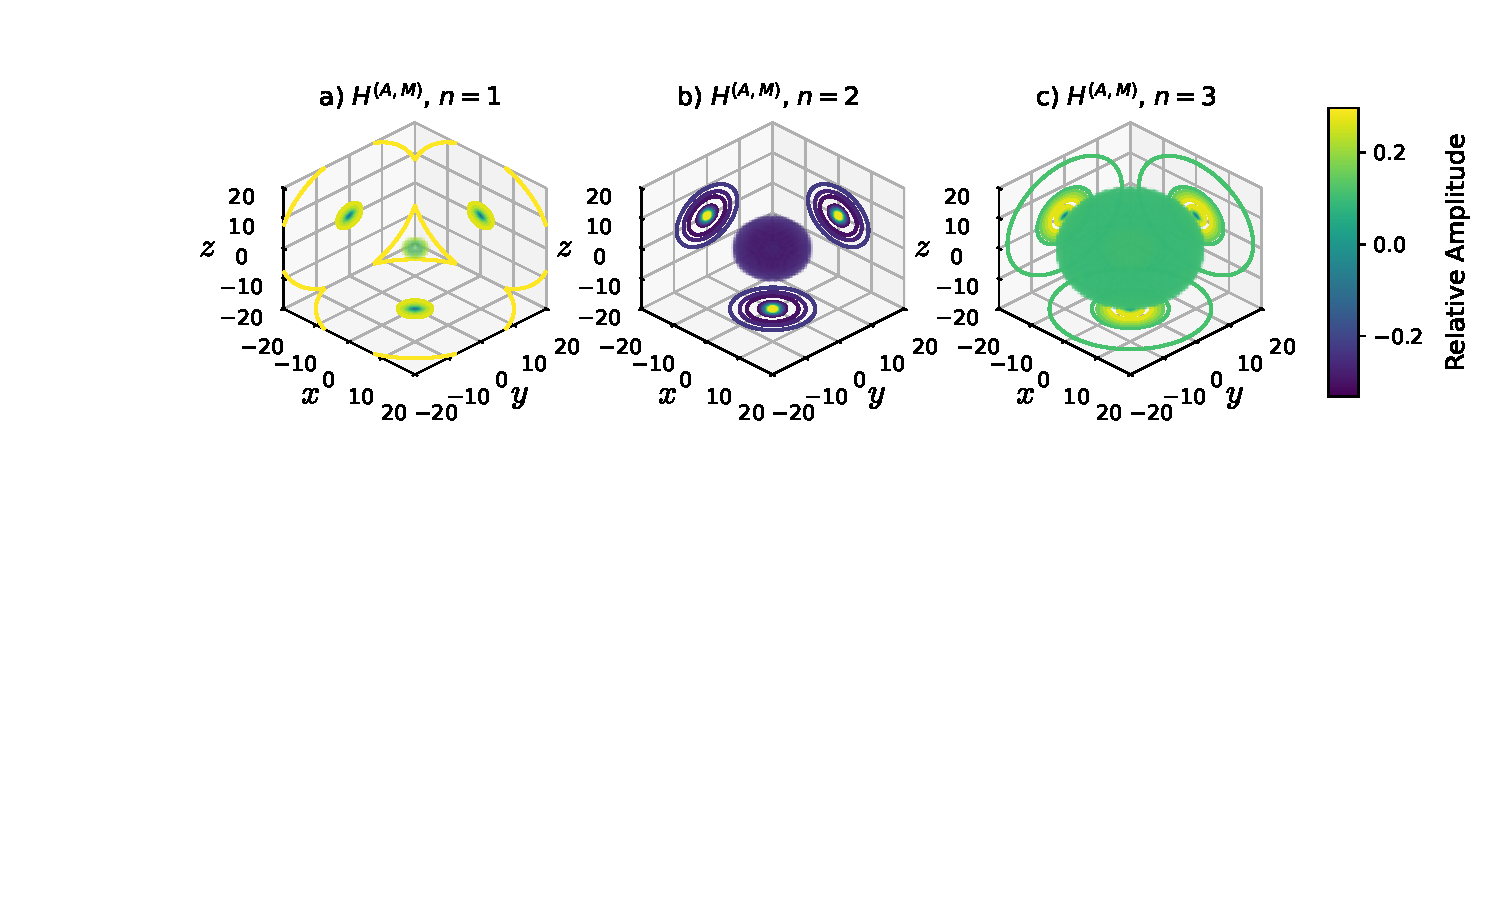
\includegraphics[width=1.2\linewidth, trim={0 0 0 1cm}, clip]{figures/HydrogenHartreeAtomicMolecular.pdf}\vspace*{-6.5cm}
\end{center}
\caption{Orbital electron wavefunctions for $l=0$, and $m=0$ Hydrogen, calculated using the atomic Hartree-Fock approximation. The molecular form of the algorithm generated identical results, and has not been included. The relative radii of these orbitals can be seen increasing with a roughly $n^2$ relationship, matching the Bohr model of a Hydrogen atom \cite{pinke_origin_2025}. Displayed using a 3D scatterplot, and filtered to display real-valued components greater than 10\% relative amplitude.}
\label{fig:hydrogenhartreeatomicmolecular}
\end{figure}

Finally, Figure \ref{fig:hydrogenhartreeanalyticalnumerical} below shows these same electron orbitals, but calculated with both the simplified atomic Hartree-Fock method, and a fully-numerical form of the general Hartree-Fock approximation. Here, the numerical wavefunctions match their analytic counterparts closely for the $n=1$ and $n=2$ states, but diverge significantly for $n=3$ and further. The first six  eigenvalue magnitudes found with this method were $|E_1|=-13.848$ $eV$, $|E_2|=-3.477$ $eV$, $|E_3|=|E_4|=-1.691$ $eV$, and $|E_5|=|E_6|=1.306$ $eV$. These values are still close to their associated Bohr-model energies, but are less accurate than the analytical Hartree-Fock results. Additionally, they diverge massively by the fifth eigenvalue, and the magnitudes $|E_3|$ through to $|E_6|$ are doubly-degenerate due to the complex-valued solutions required from the inaccurate numerical model.\\


Notably, each of these results also used a (100x100x100) resolution domain to calculate the Gaussian basis functions and resulting matrices, as smaller domain sizes such as (50x50x50) resulted in significantly inaccurate values. Additionally, the computation times of these analytic and numerical methods were compared. On one device, the analytic method took an average of $0.41s$ to complete calculations over 10 iterations, while the numerical method took an average of $2.57s$. Clearly, for $s$-type Hydrogen, the analytical method is far superior to the numerical one. However, as the wavefunctions and eigenvalues of the two lowest-energy states were both reasonably accurate, the numerical method could be useful for more complex systems or alternative basis sets, where an analytic result does not exist.


\begin{figure}[h!]
\begin{center}
\hspace*{-2.7cm}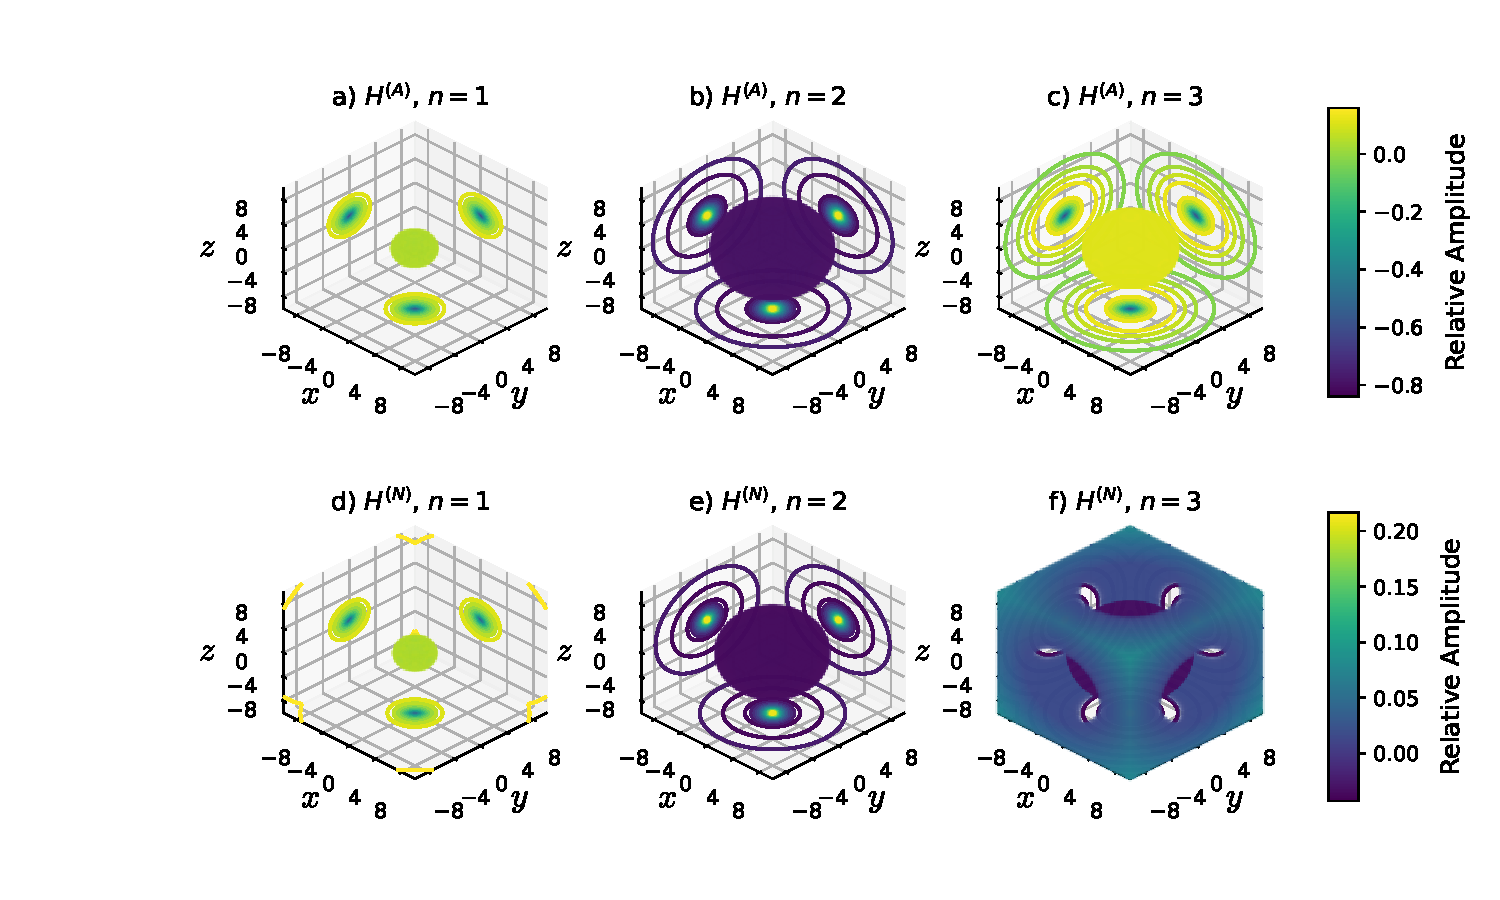
\includegraphics[width=1.2\linewidth, trim={0 0 0 1cm}, clip]{figures/HydrogenHartreeAnalyticalNumerical.pdf}\vspace*{-1cm}
\end{center}
\caption{Orbital electron wavefunctions for $l=0$, and $m=0$ Hydrogen, calculated using analytical and numerical forms of the atomic Hartree-Fock approximation. The numerical wavefunctions $H^{(N)}$ match closely with the analytical results $H^{(A)}$ for $n=1$ and $n=2$, but diverge significantly for $n=3$. Displayed using a 3D scatterplot, and filtered to display real-valued wavefunction components greater than 10\% relative amplitude.  Calculated using a domain of (100x100x100) position cells.}
\label{fig:hydrogenhartreeanalyticalnumerical}
\end{figure}


\section{Helium S-Type Orbitals}\label{sec:heliumstypestates}

\subsection{Atomic Hartree-Fock Approximation}\label{subsec:hartreeatomicresults}

Figure \ref{fig:heliumatomicelectronrepulsion} below shows the first three electron orbital wavefunctions for $s$-type ($l=0$, $m=0$) Helium, calculated with the atomic Hartree-Fock approximation, both with and without the Hartree-Fock potential $G^{(HF)}$. The wavefunctions calculated by ignoring electron-repulsion have similar shapes to those calculated for Hydrogen, and the first six eigenvalues calculated with these were $E_1=-54.417$ $eV$, $E_2=-13.605$ $eV$, $E_3=-6.047$ $eV$, $E_4=-3.401$ $eV$, $E_5=-2.176$ $eV$, and $E_6=-1.509$ $eV$. These closely match the exact values for one-electron $He^+$ Helium ions, whose energies correspond to the atom's binding energies \cite{nascimento_determination_2005}.\\

For the Helium states calculated with the Hartree-Fock potential $G^{(HF)}$ however, the resulting wavefunction amplitudes were massively high, and incorrect. As the atomic Hartree-Fock algorithm used here was tested and proven accurate for single-electron Hydrogen states, the electron-repulsion component within the algorithm must be the point of error. By comparing individual Helium matrix elements with those in the "Complex atomic exercises" document, linked to the "Quantum Chemistry Project" guide \cite{quiney_art_nodate}, it was determined that all matrix values were correct except for those from the density matrix $D_{kl}$. Unfortunately, the source of this error could not be found, despite attempts at scaling and normalising these matrix values.

\clearpage

\begin{figure}[h!]
\begin{center}
\hspace*{-2.7cm}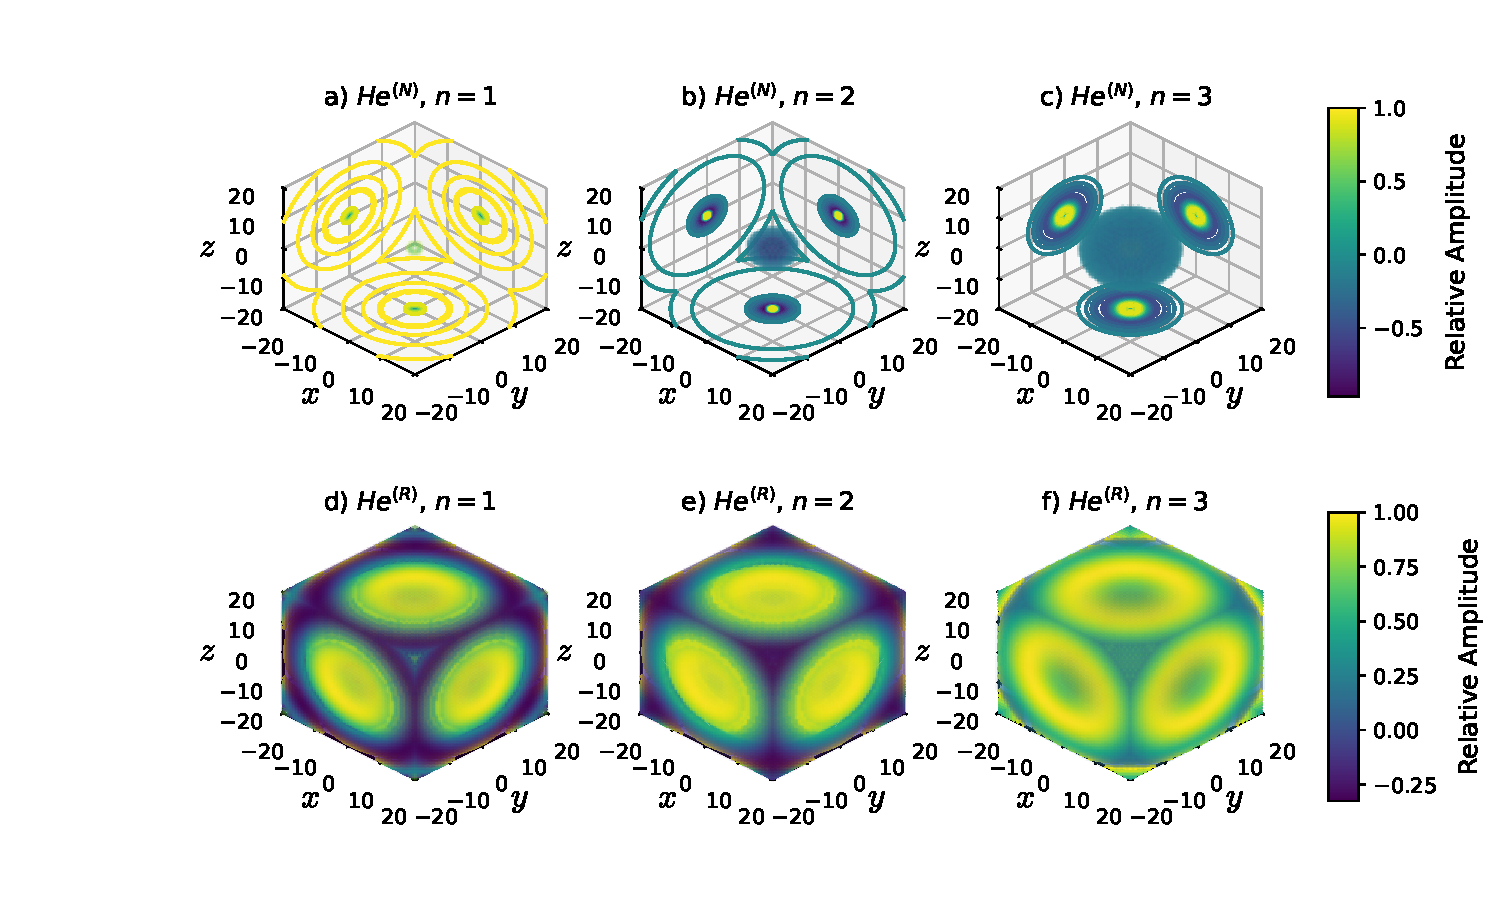
\includegraphics[width=1.2\linewidth, trim={0 0 0 1cm}, clip]{figures/HeliumAtomicElectronRepulsion.pdf}\vspace*{-1cm}
\end{center}
\caption{Orbital electron wavefunctions for $l=0$, and $m=0$ Helium, calculated using the atomic Hartree-Fock approximation, and displayed using a 3D scatterplot. The Hartree-Fock potential $G^{(HF)}$ was ignored when calculating subplots a) through c), but included for subplots d) through f). The wavefunctions calculated without electron repulsion match one-electron $He^+$ Helium states \cite{nascimento_determination_2005}, but those calculated with repulsion have incorrect, massively high amplitudes. Clearly, there is a significant error in wavefunction amplitudes produced by the electron-repulsion algorithm within this project.}
\label{fig:heliumatomicelectronrepulsion}
\end{figure}


\section{Benzene Orbitals}\label{sec:benzeneorbitals}

\subsection{Hückel Approximation}\label{subsec:huckelmethod}

Figure \ref{fig:benzenehuckelscatter} below shows orbital electron wavefunctions calculated for the six lowest-energy states of $l=1$, $m=0$ Benzene, found using the Hückel approximation. Here, the shapes of each orbital closely match existing solutions for Benzene, found both with industry-standard Hartree-Fock and density-functional calculations \cite{szwacki_aromatic_2009}, and with an analytic Hückel approximation \cite{chilton_computational_nodate}, confirming a correct algorithmic implementation. Here, the highest-energy state shows distinct, separate orbital sites around each Carbon atom in the molecule, while the lowest-energy state has electron probabilities distributed equally across the almost-circular, constant-$z$ surfaces of the Benzene ring.\\

The six eigenvalues calculated corresponding to these states were $E_1=-21.769$ $eV$, $E_2=E_3=-19.048$ $eV$, $E_4=E_5=-13.606$ $eV$, and $E_6=-10.885$ $eV$, equivalent to $\alpha \pm \beta$ or $\alpha \pm 2\beta$ for the values of $\alpha=-0.6$ and $\beta=-0.1$ chosen, in these units \cite{quiney_art_nodate}. These values do not appear to match any exact solutions, but as both $E_2$ and $E_3$, and $E_4$ and $E_5$ are doubly-degenerate, these values may be linear combinations of an exact solution \cite{quiney_art_nodate}. Notably, $E_4$ and $E_5$ are identical to the Hartree-Fock estimate for Hydrogen's ground-state energy. It is unclear whether this indicates some underlying behaviour, or is just coincidence.


\clearpage

\begin{figure}[h!]
\begin{center}
\hspace*{-2.7cm}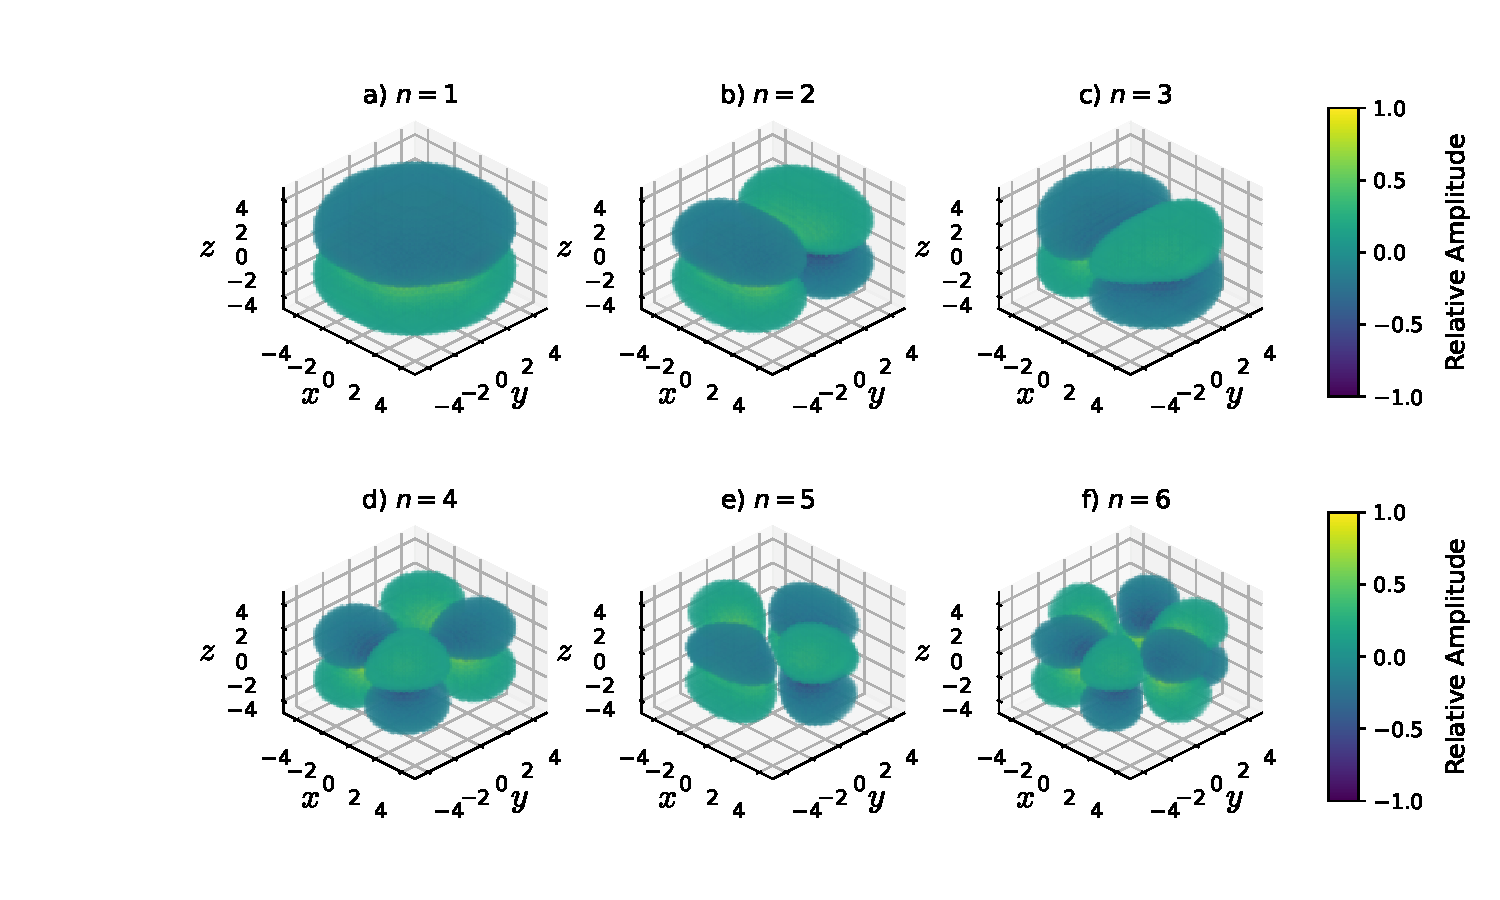
\includegraphics[width=1.2\linewidth, trim={0 0 0 1cm}, clip]{figures/BenzeneHuckelN1ToN6Scatter.pdf}\vspace*{-1cm}
\end{center}
\caption{Orbital electron wavefunctions for $l=1$, and $m=0$ Benzene, calculated using the Hückel approximation. These orbital shapes closely match known Benzene orbitals calculated through Hartree-Fock and density-functional theory \cite{szwacki_aromatic_2009}. Displayed using a 3D scatterplot, and filtered to display real-valued wavefunction components greater than 10\% relative amplitude.}
\label{fig:benzenehuckelscatter}
\end{figure}

\subsection{Hartree-Fock Molecular Approximation}\label{subsec:hartreefockmethod}

Figure \ref{fig:benzenehartreescatter} below shows orbital electron wavefunctions calculated for $l=1$, $m=0$ Benzene, using the molecular Hartree-Fock approximation. Although there is some structure to the calculated orbitals, in comparison with the Hückel method results, these are obviously incorrect. This appears to be due to the same error found earlier in the Hartree-Fock potential, $G^{(HF)}$.


\begin{figure}[h!]
\begin{center}
\hspace*{-2.7cm}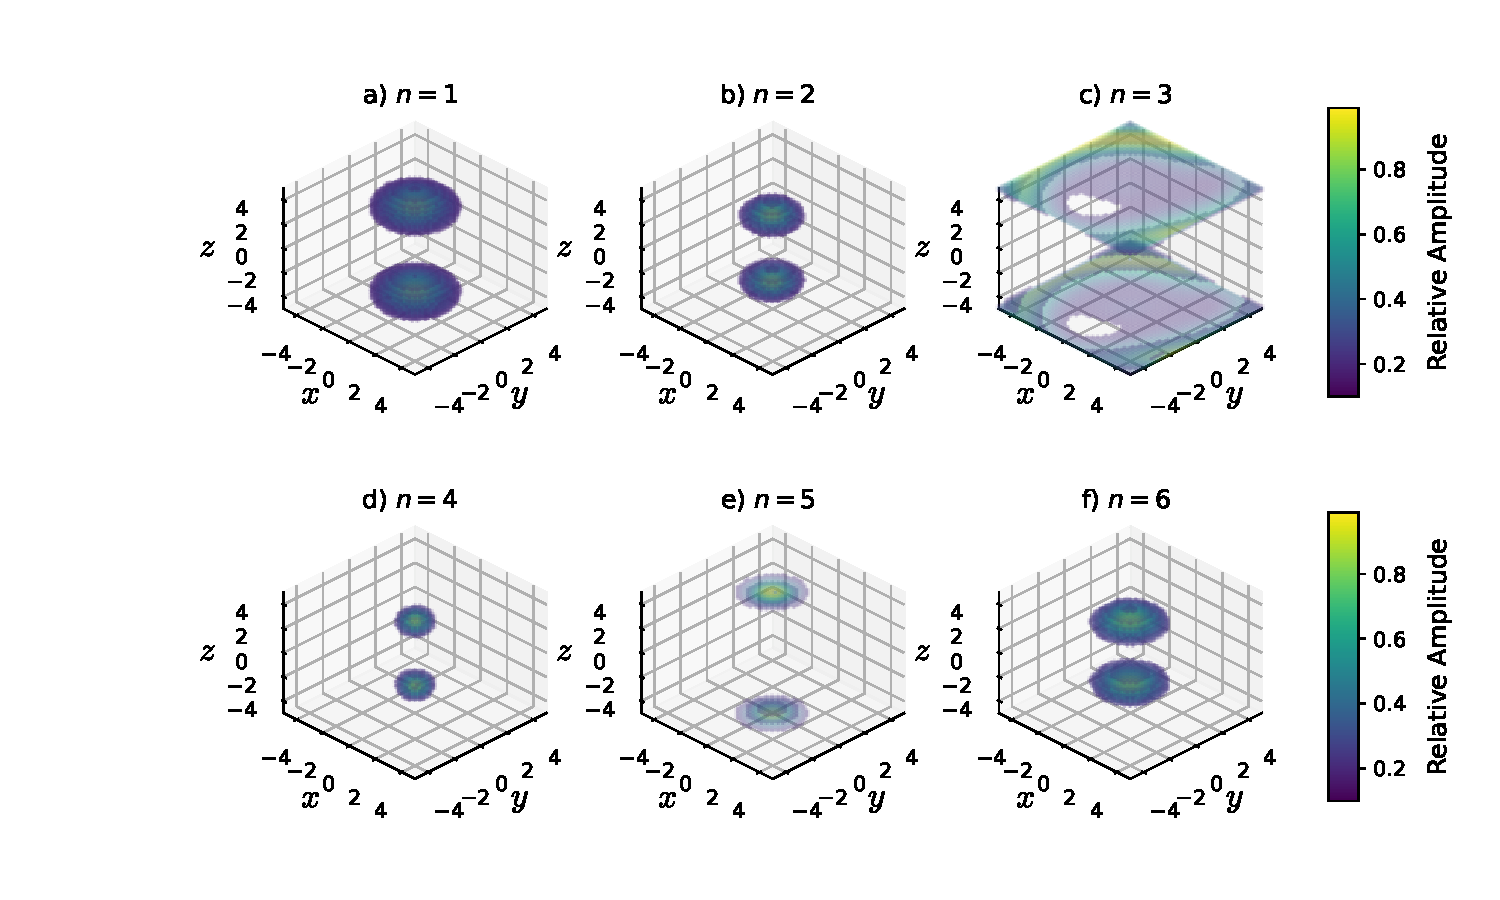
\includegraphics[width=1.2\linewidth, trim={0 7cm 0 1cm}, clip]{figures/BenzeneHartreeN1ToN6Scatter.pdf}\vspace*{-1cm}
\end{center}
\caption{Orbital electron wavefunctions for $l=1$, and $m=0$ Benzene, calculated using the molecular Hartree-Fock approximation, and displayed using a 3D scatterplot. Although there is some structure to the calculated orbitals, they are obviously incorrect. This appears to be due to the same error identified in the calculated Hartree-Fock potential $G^{(HF)}$, as seen in Figure \ref{fig:heliumatomicelectronrepulsion}.}
\label{fig:benzenehartreescatter}
\end{figure}

\clearpage


\section{Graphene Orbitals}\label{sec:grapheneorbitals}

\subsection{Hückel Approximation}\label{subsec:huckelmethod}

Figures \ref{fig:graphenehuckelscatter} and \ref{fig:graphenecontour} below show orbital electron wavefunctions calculated for evenly-spaced samples of six and three, $l=1$, $m=0$, $G_2$ Graphene states, found using the Hückel approximation. Here, the shapes of the higher-energy orbitals closely match expected behaviour for Graphene, as a periodic crystal lattice \cite{neto_electronic_2009}. The highest-energy state plotted shows distinct, separate orbital sites around each Benzene ring within the Graphene molecule. Notably, as with the molecular wavefunctions for Benzene, the lowest-energy state has electron probabilities distributed almost-equally across the entire surface of the molecule. Additionally, some of the resulting states with energies in-between these, $n=13$ and $n=17$, have interesting one-dimensional periodicity, corresponding to Benzene ring positions with the molecule.\\


\begin{figure}[h!]
\begin{center}
\hspace*{-2.7cm}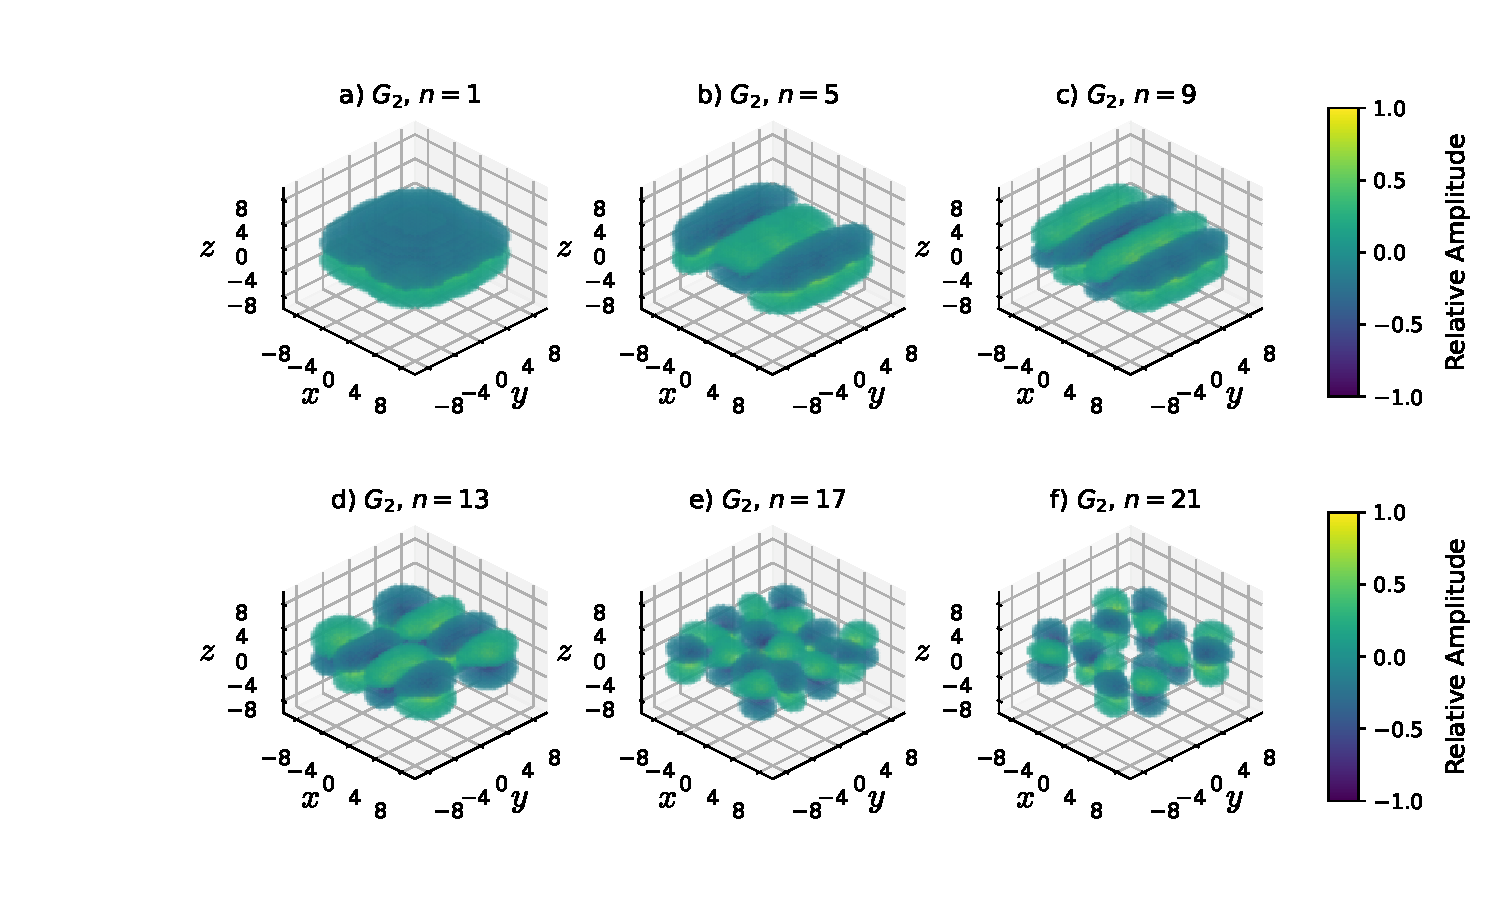
\includegraphics[width=1.2\linewidth, trim={0 0 0 1cm}, clip]{figures/GrapheneHuckelG2N1ToN21Scatter.pdf}\vspace*{-1cm}
\end{center}
\caption{Orbital electron wavefunctions for $l=1$, and $m=0$, $G_2$ Graphene, calculated using the Hückel approximation. Starting at $n=1$ and ending with $n=21$, every fourth energy state is displayed using a 3D scatterplot of the wavefunction, to showcase a greater variety of Graphene orbitals. These match the periodic structure expected from Graphene's 2D crystal lattice, with the higher-energy orbitals appearing periodic over the Graphene crystal's unit cell \cite{neto_electronic_2009}. Filtered to display real-valued wavefunction components greater than 10\% relative amplitude.}
\label{fig:graphenehuckelscatter}
\end{figure}
\clearpage



\begin{figure}[h!]
\begin{center}
\hspace*{-2.7cm}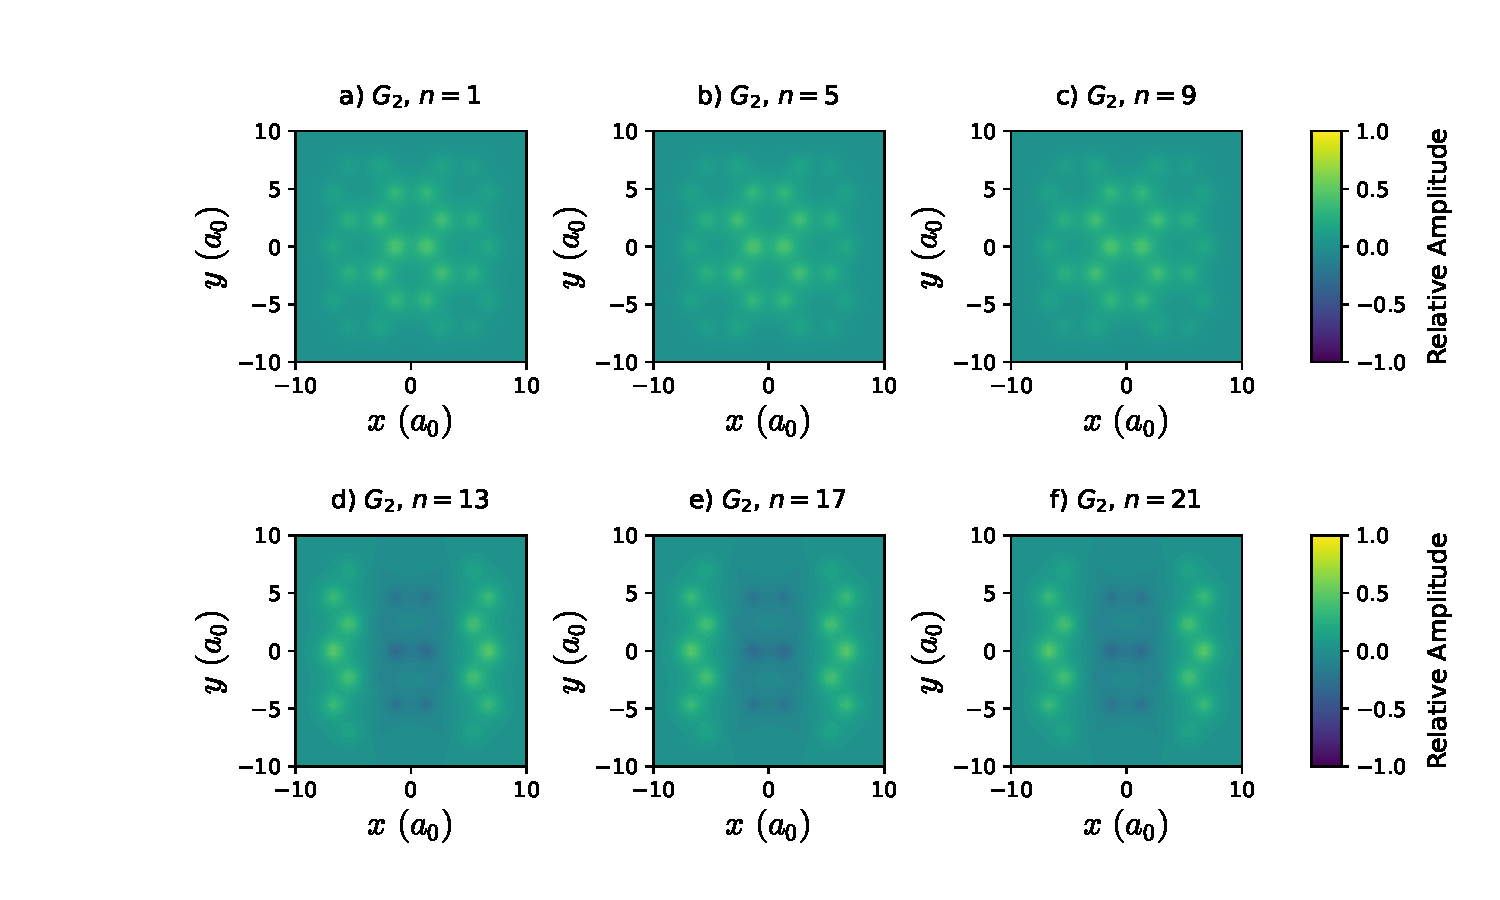
\includegraphics[width=1.2\linewidth, trim={0 7cm 0 1cm}, clip]{figures/GrapheneG2N1ToN21Contour.pdf}\vspace*{-1cm}
\end{center}
\caption{Orbital electron wavefunctions for $l=1$, and $m=0$, $G_2$ Graphene, calculated using the Hückel approximation. Starting at $n=1$ and ending with $n=9$, every fourth energy state is displayed using a $z=0$, 2D contour of the 3D wavefunction, to showcase a greater variety of Graphene orbitals. With this particular 2D slice, the atomic structure of the Graphene crystal is quite visible.}
\label{fig:graphenecontour}
\end{figure}

Finally, Figure \ref{fig:graphenehuckelG1G2G3} below shows the highest-energy ($n=15$, $n=28$, and $n=60$) states for the three Graphene molecules $G_1$, $G_2$, and $G_3$, respectively. These show that the periodic structure of the orbital wavefunctions calculated is consistent across molecule sizes, but displays slightly different amplitudes and shapes at the boundaries of each molecule. For a much larger Graphene molecule, it would then be sufficient to model the electron wavefunctions and probabilities periodically, using a Fourier-transformed reciprocal lattice of the spatial lattice used here \cite{neto_electronic_2009}. This could be interesting further study, as the reciprocal lattice can be described with less information than its spatial counterpart, and could be simulated with much higher resolutions (albeit without this form of the Hückel approximation).


\begin{figure}[h!]
\begin{center}
\hspace*{-2.7cm}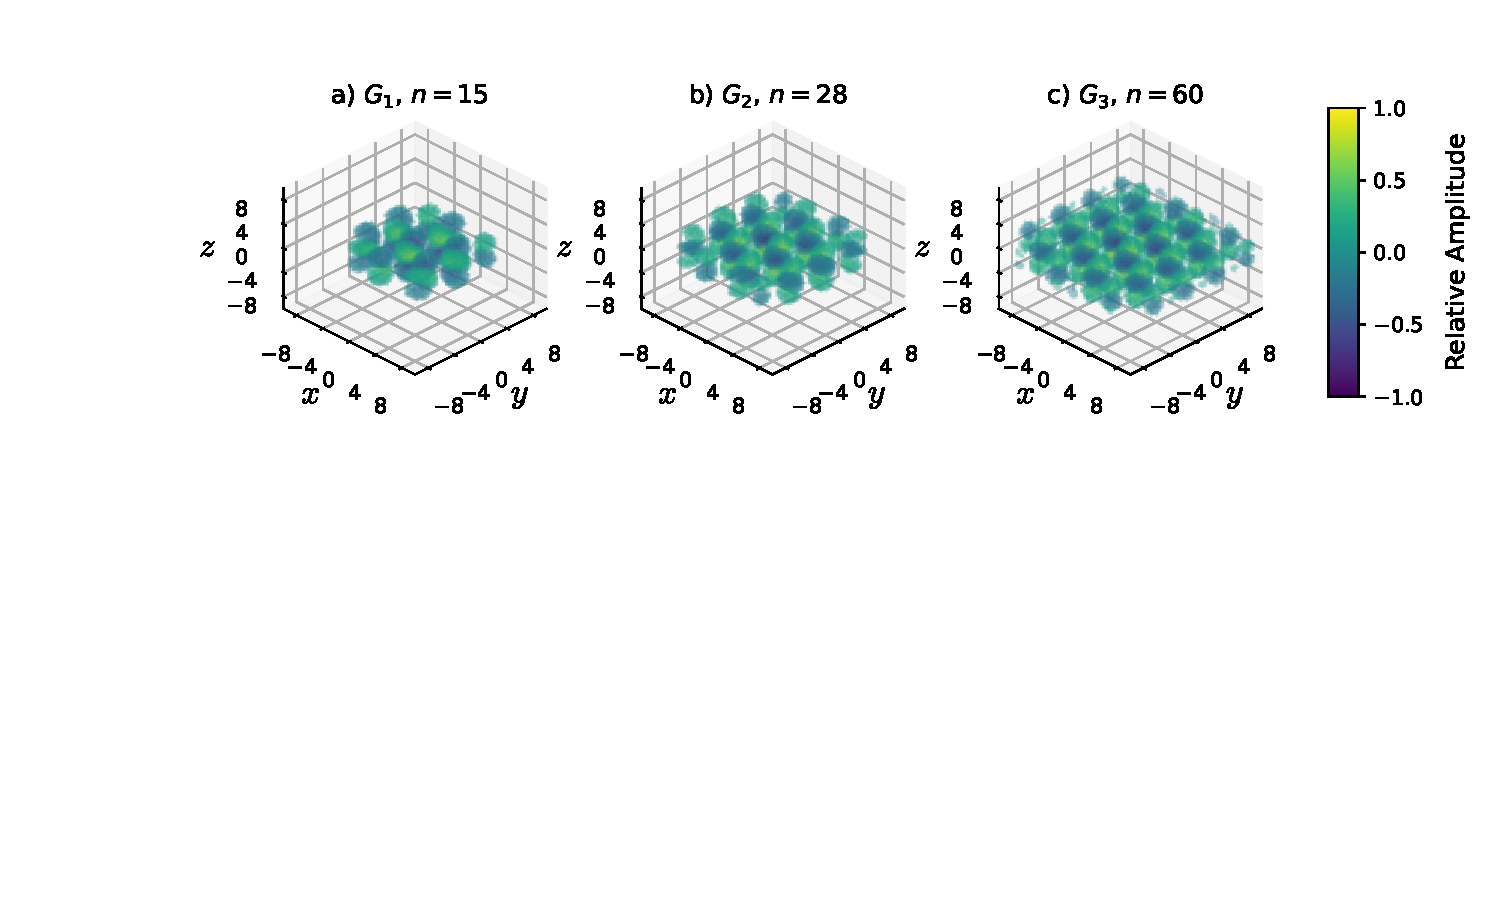
\includegraphics[width=1.2\linewidth, trim={0 0 0 1cm}, clip]{figures/GrapheneHuckelG1G2G3.pdf}\vspace*{-6.5cm}
\end{center}
\caption{The highest-energy orbital electron wavefunctions of $G_1$, $G_2$, and $G_3$ Graphene, calculated using the Hückel approximation. These each match the periodic structure expected from Graphene's 2D crystal lattice \cite{neto_electronic_2009}. Filtered to display real-valued wavefunction components greater than 10\% relative amplitude.}
\label{fig:graphenehuckelG1G2G3}
\end{figure}


\subsection{Hartree-Fock Molecular Approximation}\label{subsec:hartreefockmethod}

The $G_2$ electron orbitals were also calculated using the molecular Hartree-Fock approximation, but had no visible structure due to the electron-repulsion error discussed earlier, and thus are not plotted. These calculations are more good candidates for further study, as the molecular Hartree-Fock method considered more complicated electron-electron energy contributions \cite{quiney_art_nodate}, and could display significant deviations from the Hückel method results, particularly at the molecular boundaries.